\documentclass[12pt]{letter}
\usepackage{amsmath,amsfonts,amsthm,amstext,amssymb,graphicx, multicol,fancyhdr,lastpage,fullpage,framed,fancybox,enumerate,tikz,color,mathrsfs, polynom, pifont}
\usepackage[margin=0.6in,headsep=3pt, headheight=15pt]{geometry}

% ----------------------------------------------------------
% Custom Definitions, Commands, Environments, etc.

% Sets of numbers
\def\R{\mathbb{R}} % The reals
\def\N{\mathbb{N}} % The naturals
\def\Z{\mathbb{Z}} % The integers
\def\Q{\mathbb{Q}} % The rationals

% Blank space
\newcommand{\blank}[1]{\underline{\hspace{#1}}} % Blank space

% Change font colors
\newcommand{\cyan}[1]{{\color{cyan}{#1}}} % Changes font to cyan
\newcommand{\red}[1]{{\color{red}{#1}}} % Changes font to red
\newcommand{\magenta}[1]{{\color{magenta}{#1}}} % Changes font to magenta
\newcommand{\orange}[1]{{\color{orange}{#1}}} % Changes font to orange
\newcommand{\yellow}[1]{{\color{yellow}{#1}}} % Changes font to yellow
\newcommand{\violet}[1]{{\color{violet}{#1}}} % Changes font to violet
\newcommand{\green}[1]{{\color{green}{#1}}} % Changes font to green
\newcommand{\blue}[1]{{\color{blue}{#1}}} % Changes font to blue
\newcommand{\white}[1]{{\color{white}{#1}}} % Changes font to white

% Fitted inclusion symbols
\newcommand{\fp}[1]{\left({#1}\right)} % Fitted parentheses around content
\newcommand{\fb}[1]{\left[{#1}\right]} % Fitted brackets
\newcommand{\set}[1]{\left\{{#1}\right\}} % Fitted braces (useful for sets)
\newcommand{\av}[1]{\left|{#1}\right|} % Fitted absolute value bars

% Augmented Matrix Environment
\newenvironment{amatrix}[1]{%
	\left[\begin{array}{@{}*{#1}{c}|c@{}}
	}{%
	\end{array}\right]
}

% Miscellaneous
\def\then{\Rightarrow}
\def\to{\rightarrow}
\def\d{^{\circ}}
\newcommand{\?}{\stackrel{?}{=}}
\newcommand{\cmark}{\text{ \ding{51}}}
\newcommand{\xmark}{\text{ \ding{55}}}



% Coordinate Plane (Four-Quadrant)
\def\coordplane {
	\begin{tikzpicture}		\draw[step=0.25cm,black,very thin,opacity=0.25] (-2.5cm, -2.5cm) grid (2.5cm, 2.5cm);
	\draw[<->,thick,black] (-2.5cm, 0) -- (2.5cm, 0) node[anchor=north west,pos=0.94,font=\scriptsize]{$x$};
	\draw[<->,thick,black] (0,-2.5cm) -- (0, 2.5cm) node[anchor=south east,font=\scriptsize,pos=0.94]{$y$};
	\end{tikzpicture}
}

% Coordinate Plane (One-Quadrant)
\def\onequad {
	\begin{tikzpicture}
	\draw[step=0.25cm, black, very thin, opacity=0.25] (0,0) grid (7.5cm,5cm);
	\draw[->, thick, black] (0,0) -- (7.5cm, 0) node[anchor=north west,font=\scriptsize,pos=0.94]{$x$};
	\draw[->, black, thick] (0,0) -- (0,5cm) node[anchor=south east,font=\scriptsize,pos=0.94]{$y$};
	\end{tikzpicture}
}

% Counters
\newcounter{exercise}

% Exercise environment (auto-numbered)
\newenvironment{exercise}[1][]{\begin{framed}\refstepcounter{exercise}\textbf{Exercise~\theexercise:} #1}{\end{framed}}

% Book exercise environment
\newenvironment{bex}[2][] {
	\begin{framed}
		\textbf{Book Exercise {#2}}#1
	\end{framed}
}
% ----------------------------------------------------------

% ----------------------------------------------------------
% Header and Footer Information
% \pagestyle{fancy}
% \fancyhf{}
% \renewcommand{\headrulewidth}{0pt}
% \rhead{Name: \blank{2in}}
% \lhead{@}
% \rfoot{Page \thepage \, of \,\pageref{LastPage}}
% ----------------------------------------------------------
\author{Jacob Ayers}

\begin{document}
	\textbf{Assignment 11 Key \\ MAT 130}
	
	\begin{bex}{9.1.6}
		{
			
		}
	\end{bex} \vspace{-8pt}
	
	% My answer here
	(a) $4(2)^2 + (-13) = 4(4) - 13 = 3 \cmark \\ -(2) - (-13) = -2 + 13 = 11 \cmark$ \\ $(2, -13)$ is a solution to the system.
	
	(b) $4(1)^2 + (-2) = 4 - 2 = 2 \xmark$ \\ $(1, -2)$ is not a solution to the system.
	
	(c) $4\fp{-\dfrac32}^2 + \fp{-\dfrac{31}{3}} = 9 - \dfrac{31}{3} = -\dfrac43 \xmark$ \\ $\fp{-\dfrac32, -\dfrac{31}{3}}$ is not a solution to the system.
	
	(d) $4\fp{-\dfrac74}^2 + \fp{-\dfrac{37}{4}} = \dfrac{49}{4} - \dfrac{37}{4} = 3 \cmark \\ -\fp{-\dfrac74} - \fp{-\dfrac{37}{4}} = \dfrac74 + \dfrac{37}{4} = 11 \cmark$ \\ $\fp{-\dfrac74, -\dfrac{37}{4}}$ is a solution to the system.
	
	\vfill % \newpage
	
	\begin{bex}{9.1.16}
		{
			
		}
	\end{bex} \vspace{-8pt}
	
	% My answer here
	We can easily isolate $y$ in the top equation: $y = -2x + 9$. Now, we can substitute this value of $y$ into the bottom equation to solve for $x$: \begin{flalign*}
	3x - 5(-2x + 9) &= 20 & \\
	3x + 10x - 45 &= 20 & \\
	13x &= 65 & \\
	x &= 5 & \\
	y &= -2(5) + 9 & \\
	&= -1
	\end{flalign*}
	The solution is $\fp{5, -1}$.
	
	
	\vfill \newpage
	
	\begin{bex}{9.1.18}
		{
			
		}
	\end{bex} \vspace{-8pt}
	
	% My answer here
	We can easily isolate $x$ in the bottom equation: $x = -2y + 4$. Now, we can substitute this value of $x$ into the top equation to solve for $y$: \begin{flalign*}
	6\fp{-2y + 4} - 3y - 4 &= 0 & \\
	-12y + 24 - 3y - 4 &= 0 & \\
	-15y + 20 &= 0 & \\
	-15y &= -20 & \\
	y &= \dfrac{-20}{-15} = \dfrac43 & \\
	x &= -2\fp{\dfrac43} + 4 & \\
	&= -\dfrac83 + \dfrac{12}{3} & \\
	&= \dfrac43
	\end{flalign*}
	The solution is $\fp{\dfrac43, \dfrac43}$.
	
	\vfill % \newpage
	
	\begin{bex}{9.1.20}
		{
			
		}
	\end{bex} \vspace{-8pt}
	
	% My answer here
	Solving for $y$ in the top equation: $y = -0.5x - 3.5$. Substituting and solving: \begin{flalign*}
	x - 3.2\fp{-0.5x - 3.5} &= 3.4 & \\
	x + 1.6x + 11.2 &= 3.4 & \\
	2.6x &= -7.8 & \\
	x &= -3 & \\
	y &= -0.5(-3) - 3.5 & \\
	&= 1.5 - 3.5 & \\
	&= -2
	\end{flalign*}
	The solution is $(-3, -2)$.
	
	\vfill \newpage
	
	\begin{bex}{9.1.30}
		{
			
		}
	\end{bex} \vspace{-8pt}
	
	% My answer here
	Solving the top equation for $x$: $x = 2y$. Substituting and solving: \begin{flalign*}
	3(2y) - y^2 &= 0 & \\
	-y^2 + 6y &= 0 & \\
	-y\fp{y - 6} &= 0 & \\
	y &= \set{0, 6} & \\
	x &= 2(0) = 0 & \\
	x &= 2(6) = 12 & \\
	\end{flalign*}
	There are two solutions. They are $(0, 0)$ and $(12, 6)$.
	
	\vfill % \newpage
	
	\begin{bex}{9.1.32}
		{
			
		}
	\end{bex} \vspace{-8pt}
	
	% My answer here
	Since both equations already have $y$ isolated, we can set the right sides of the equations equal to one another to solve for $x$: \begin{flalign*}
	-x &= x^3 + 3x^2 + 2x & \\
	x^3 + 3x^2 + 3x &= 0 & \\
	x\fp{x^2 + 3x + 3} &= 0 & \\
	x &= 0 & \\
	x &= \dfrac{-3\pm\sqrt{3^2 - 4(1)(3)}}{2(1)} & \\
	&= \dfrac{-3 + \sqrt{-3}}{2} \xmark & \\
	y &= -0 = 0
	\end{flalign*}
	We do not consider imaginary solutions. The only solution is $(0, 0)$.
	
	\vfill \newpage
	
	\begin{bex}{9.1.34}
		{
			
		}
	\end{bex} \vspace{-8pt}
	
	% My answer here
	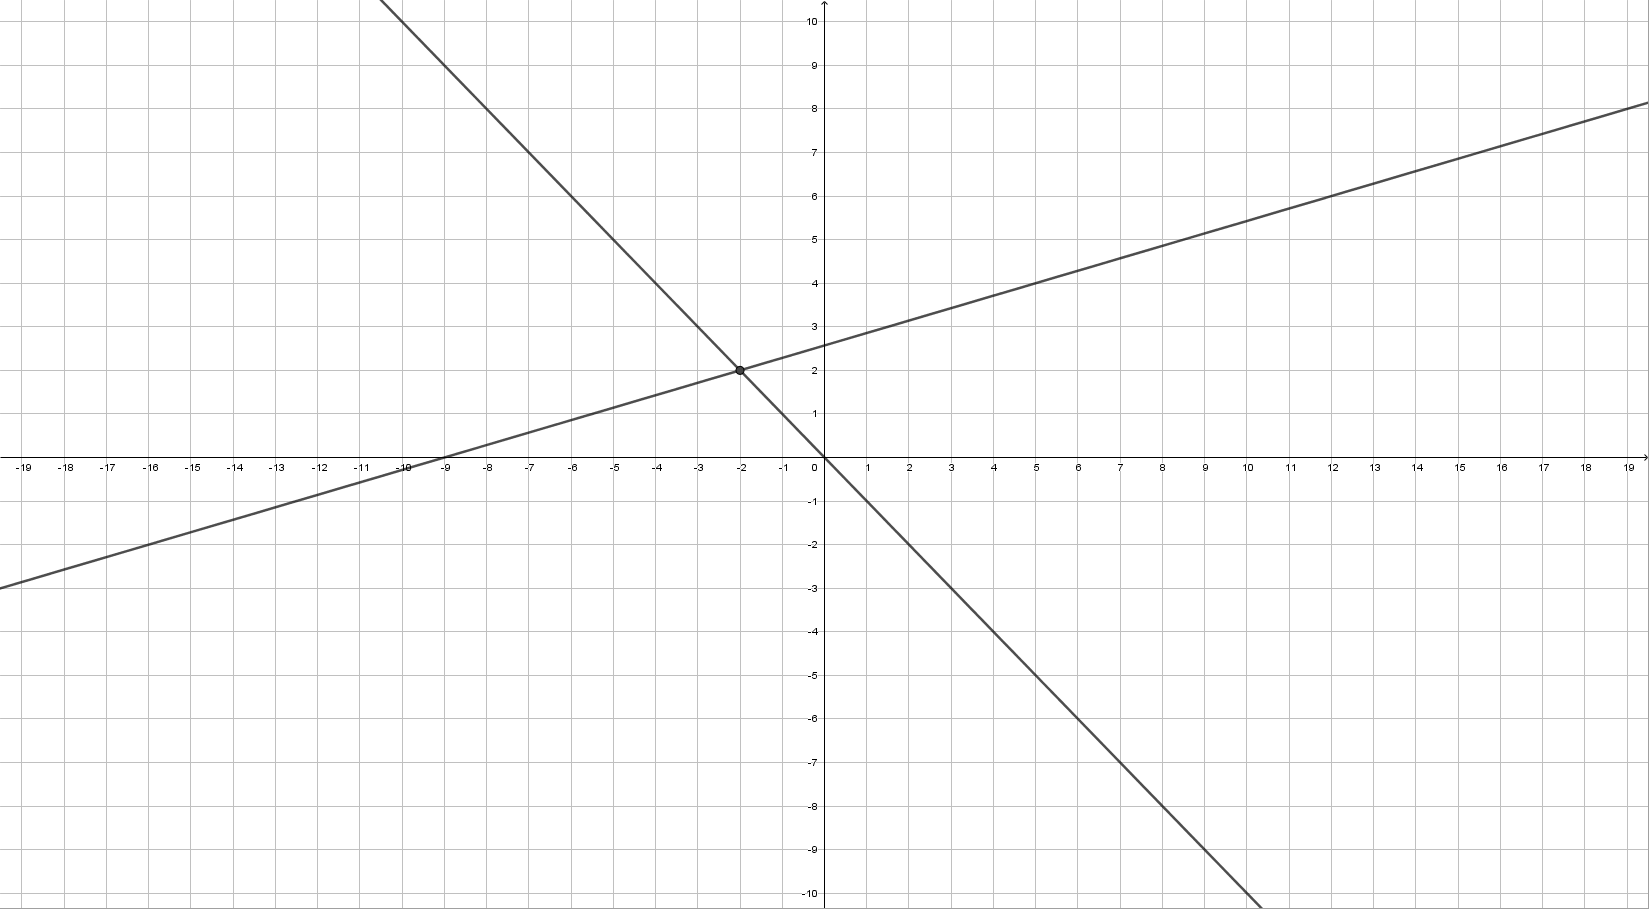
\includegraphics[width=3in]{9134.png}
	
	The solution is $(-2, 2)$.
	
	\vfill % \newpage
	
	\begin{bex}{9.1.60}
		{
			
		}
	\end{bex} \vspace{-8pt}
	
	% My answer here
	Using GeoGebra, we find two equilibrium points: $(16.68, 1.49)$ and $(53.55, 1.85)$.
	
	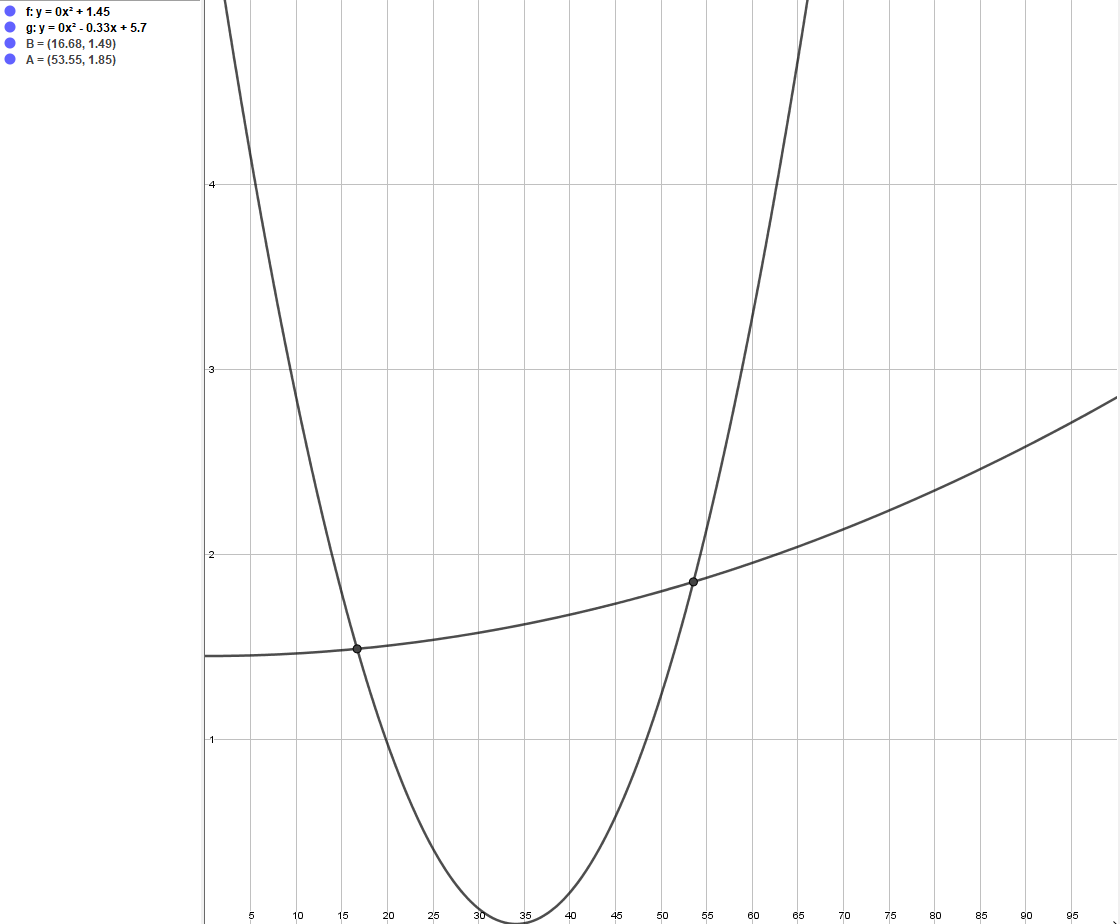
\includegraphics[width=3in]{9160.png}
	
	\vfill \newpage
	
	\begin{bex}{9.1.64}
		{
			
		}
	\end{bex} \vspace{-8pt}
	
	% My answer here
	Recall that the perimeter of a rectangle is found using the formula $p = 2\ell + 2w$. We need to solve the system $\begin{cases}
	2\ell + 2w = 42 \\ w = \dfrac34 \ell
	\end{cases}$ \begin{flalign*}
	2\ell + 2\fp{\dfrac34 \ell} &= 42 & \\
	2\ell + \dfrac32 \ell &= 42 & \\
	\dfrac{7}{2}\ell &= 42 & \\
	\ell &= 12 & \\
	w &= \dfrac34\fp{12} &= 9
	\end{flalign*}
	The rectangle is 9 inches $\times$ 12 inches.
	
	\vfill % \newpage
	
	\begin{bex}{9.2.14}
		{
			
		}
	\end{bex} \vspace{-8pt}
	
	% My answer here
	If we add the two equations together, $y$ will be eliminated. Solving for $x$:
	
	$5x = 30 \then x = 6$
	
	Now, back-substituting into the bottom equation: \begin{flalign*}
	2(6) + 5y &= 22 & \\
	12 = 5y &= 22 & \\
	5y &= 10 & \\
	y &= 2
	\end{flalign*}
	The solution is $(6, 2)$.
	
	\vfill \newpage
	
	\begin{bex}{9.2.18}
		{
			
		}
	\end{bex} \vspace{-8pt}
	
	% My answer here
	Multiply the top equation by $-8$ to eliminate $r$:
	
	$\begin{cases}
	-16r - 32s = -40 \\ 16r + 50s = 55
	\end{cases}$
	$18s = 15 \then s = \dfrac56$
	
	Back-substitute into the original top equation: \begin{flalign*}
	2\fp{\dfrac56} + 4s &= 5 & \\
	4s + \dfrac53 &= 5 & \\
	4s &= \dfrac{10}{3} & \\
	s &= \dfrac{10}{12} = \dfrac56
	\end{flalign*}
	The solution is $\fp{\dfrac56, \dfrac56}$.
	
	\vfill % \newpage
	
	\begin{bex}{9.2.22}
		{
			
		}
	\end{bex} \vspace{-8pt}
	
	% My answer here
	Multiply the top equation by $-5$ and the bottom equation by $2$ to eliminate $x$:
	
	$\begin{cases}
		-10x - 25y = -40 \\ 10x + 16y = 20
	\end{cases}$
	$-9y = -20 \then y = \dfrac{20}{9}$
	
	Back-substitute into the original top equation: \begin{flalign*}
	2x + 5\fp{\dfrac{20}{9}} &= 8 & \\
	2x + \dfrac{100}{9} &= 8 & \\
	2x &= -\dfrac{28}{9} & \\
	x &= -\dfrac{14}{9}
	\end{flalign*}
	The solution is $\fp{-\dfrac{14}{9}, \dfrac{20}{9}}$.
	
	
	\vfill \newpage
	
	\begin{bex}{9.2.26}
		{
			
		}
	\end{bex} \vspace{-8pt}
	
	% My answer here
	Multiply the top equation by $5$ and the bottom equation by $2$:
	
	$\begin{cases}
	-30x + 20y = 35 \\ 30x - 20y = -32
	\end{cases}$
	$0 = 3$
	
	There is no solution to this system.
	
	\vfill % \newpage
	
	\begin{bex}{9.2.30}
		{
			
		}
	\end{bex} \vspace{-8pt}
	
	% My answer here
	It will be easier to solve this system if we first make it so that the top equation no longer has fractions. This can be accomplished by multiplying the equation by $6$: \begin{flalign*}
	6\fp{\dfrac{x-1}{2} + \dfrac{y+2}{3}} &= 6(4) & \\
	3(x-1) + 2(y+2) &= 24 & \\
	3x - 3 + 2y + 4 &= 24 & \\
	3x + 2y + 1 &= 24 & \\
	3x + 2y &= 23
	\end{flalign*}
	Now, the two equations can be added together and $y$ will be eliminated.
	
	$\begin{cases}
	3x + 2y = 23 \\ x - 2y = 5
	\end{cases}$
	$4x = 28 \then x = 7$
	
	So $7 - 2y = 5 \then y = 1$. The solution is $(7,1)$.
	
	\vfill % \newpage
	
	\begin{bex}{9.2.36}
		{
			
		}
	\end{bex} \vspace{-8pt}
	
	% My answer here
	Either algebraic method would be pretty straightforward; I'll choose to use elimination since we only need to multiply the top equation by $-1$ in order to eliminate $y$.
	
	$\begin{cases}
	x - 3y = -17 \\ 4x + 3y = 7
	\end{cases}$
	$5x = -10 \then x = -2$
	\begin{flalign*}
	-(-2) + 3y &= 17 & \\
	3y + 2 &= 17 & \\
	3y &= 15 & \\
	y &= 5
	\end{flalign*}
	The solution is $(-2, 5)$.
	
	\vfill \newpage
	
	\begin{bex}{9.2.38}
		{
			
		}
	\end{bex} \vspace{-8pt}
	
	% My answer here
	Since $y$ is already isolated in the bottom equation, we should solve the system using substitution. \begin{flalign*}
	-5x + 9(x-4) &= 13 & \\
	-5x + 9x - 36 &= 13 & \\
	4x &= 49 & \\
	x &= \dfrac{49}{4} & \\
	y &= \dfrac{49}{4} - 4 & \\
	&= \dfrac{49}{4} - \dfrac{16}{4} & \\
	&= \dfrac{33}{4}
	\end{flalign*}
	The solution is $\fp{\dfrac{49}{4}, \dfrac{33}{4}}$.
	
	\vfill % \newpage
	
	\begin{bex}{9.2.40}
		{
			
		}
	\end{bex} \vspace{-8pt}
	
	% My answer here
	Since $y$ is isolated in both equations, we should solve this system using substitution. \begin{flalign*}
	-3x - 8 &= 15 - 2x & \\
	-x - 8 &= 15 & \\
	-x &= 23 & \\
	x &= -23 & \\
	y &= 15 - 2(-23) & \\
	&= 15 + 46 & \\
	&= 61
	\end{flalign*}
	The solution is $(-23, 61)$.
	
	\vfill \newpage
	
	\begin{bex}{9.3.8}
		{
			
		}
	\end{bex} \vspace{-8pt}
	
	% My answer here
	(a) $3(3) + 4(-1) - 2 = 9 - 4 - 2 = 3 \xmark$ \\
	$(3, -1, 2)$ is not a solution to the system.
	
	(b) $3(1) + 4(3) - (-2) = 3 + 12 + 2 = 17 \cmark \\ 5(1) - 3 + 2(-2) = 5 - 3 - 4 = -2 \cmark \\ 2(1) - 3(3) + 7(-2) = 2 - 9 - 14 = -21 \cmark \\ (1, 3, -2)$ is a solution to the system.
	
	(c) $3(1) + 4(5) - 6 = 3 + 20 - 6 = 17 \cmark \\ 5(1) - 5 + 2(6) = 5 - 5 + 12 = 12 \xmark \\ (1,5,6)$ is not a solution to the system.
	
	(d) $3(1) + 4(-2) - 2 = 3 - 8 - 2 = -7 \xmark \\ (1, -2, 2)$ is not a solution to the system.
	
	\vfill % \newpage
	
	\begin{bex}{9.3.12}
		{
			
		}
	\end{bex} \vspace{-8pt}
	
	% My answer here
	This system is in row-echelon form, so we can work our way up the system using back-substitution.
	
	$y - (-1) = 8 \then y = 7$
	
	$x - 2(7) + 2(-1) = 20 \then x - 16 = 20 \then x = 36$
	
	The solution is $(36, 7, -1)$.
	
	\vfill \newpage
	
	\begin{bex}{9.3.24}
		{
			
		}
	\end{bex} \vspace{-8pt}
	
	% My answer here
	First, eliminate $x$ from the middle equation by multiplying the top equation by $-1$ and adding it to the middle equation:
	
	$\begin{cases}
	-x - y - z &= -5 \\ x - 2y + 4z &= 13 \\ 3y + 4z &= 13
	\end{cases} \then \begin{cases}
	x + y + z &= 5 \\ -3y + 3z &= 8 \\ 3y + 4z &= 13
	\end{cases}$
	
	Now, add the middle equation to the bottom equation to eliminate $y$ in the bottom equation:
	
	$\begin{cases}
	x + y + z &= 5 \\ -3y + 3z &= 8 \\ 7z &= 21
	\end{cases}$
	
	The bottom equation simplifies to $z = 3$. The system is in row-echelon form, so we can use back-substitution to find the values of the other variables.
	
	$-3y + 3(3) = 8 \then -3y = -1 \then y = \dfrac13$ \\
	$x + \dfrac13 + 3 = 5 \then x + \dfrac{10}{3} = \dfrac{15}{3} \then x = \dfrac{5}{3}$ \\
	Solution is $\fp{\dfrac53, \dfrac13, 3}$
	
	\vfill % \newpage
	
	\begin{bex}{9.3.28}
		{
			
		}
	\end{bex} \vspace{-8pt}
	
	% My answer here
	First, multiply the top equation by $2$, the middle equation by $-5$, and the bottom equation by $-10$. We can then add the top equation and the middle equation to eliminate $x$ in the middle equation, and add the top equation and the bottom equation to eliminate $x$ in the bottom equation.
	
	$\begin{cases}
	10x - 6y + 4z &= 6 \\ -10x - 20y + 5z &= -35 \\ -10x + 110y - 40z &= -30
	\end{cases} \then \begin{cases}
	5x - 3y + 2z &= 3 \\ -26y + 9z &= -29 \\ 104y - 36z &= -24
	\end{cases}$
	
	Next, multiply the middle equation by $4$ and add it to the bottom equation; this eliminates both $y$ and $z$ in the bottom equation.
	
	$\begin{cases}
	5x - 3y + 2z &= 3 \\ -104y + 36z &= -116 \\ 104y - 36z &= -24
	\end{cases} \then \begin{cases}
	5x - 3y + 2z &= 3 \\ -26y + 9z &= -29 \\ 0 &= -140
	\end{cases}$
	
	The bottom equation is false, so this system of equations has no solution.
	
	\vfill \newpage
	
	\begin{bex}{9.3.32}
		{
			
		}
	\end{bex} \vspace{-8pt}
	
	% My answer here
	First, multiply the top equation by $-5$, the middle equation by $4$, and the bottom equation by $5$. We can then add the top equation to the middle equation to eliminate $x$ in the middle equation, and add the top equation to the bottom equation to eliminate $x$ in the bottom equation.
	
	$\begin{cases}
	-20x - 15y - 85z &= 0 \\ 20x + 16y + 88z &= 0 \\ 20x + 10y + 95z &= 0
	\end{cases} \then \begin{cases}
	4x + 3y + 17z &= 0 \\ y + 3z &= 0 \\ -5y + 10z &= 0
	\end{cases}$
	
	Next, multiply the bottom equation by $\dfrac15$ and add the second equation to it to eliminate $y$ in the bottom equation.
	
	$\begin{cases}
	4x + 3y + 17z &= 0 \\ y + 3z &= 0 \\ -y + 2z &= 0
	\end{cases} \then \begin{cases}
	4x + 3y + 17z &= 0 \\ y + 3z &= 0 \\ 5z &= 0
	\end{cases}$
	
	The bottom equation simplifies to $z = 0$. We can now find the values of the other two variables using back-substitution.
	
	$y + 3(0) = 0 \then y = 0$ \\
	$4x + 3(0) + 17(0) = 0 \then x = 0$ \\
	Solution is $(0, 0, 0)$
	
	\vfill \newpage
	
	\begin{bex}{9.3.38}
		{
			
		}
	\end{bex} \vspace{-8pt}
	
	% My answer here
	First, multiply the middle equation by $-\dfrac12$. We can then add the top equation to the middle equation to eliminate $x$ in the middle equation and add the top equation to the bottom equation to eliminate $x$ in the bottom equation.
	
	$\begin{cases}
	2x + y - 3z &= 4 \\ -2x - z &= -5 \\ -2x + 3y - 13z &= -8
	\end{cases} \then \begin{cases}
	2x + y - 3z &= 4 \\ y - 4z &= -1 \\ 4y - 16z &= -4 
	\end{cases}$
	
	Now, multiply the bottom equation by $-\dfrac14$ and add the middle equation to the bottom equation; this will eliminate $y$ and $z$ in the bottom equation.
	
	$\begin{cases}
	2x + y - 3z &= 4 \\ y - 4z &= -1 \\ -y + 4z &= 1
	\end{cases} \then \begin{cases}
	2x + y - 3z &= 4 \\ y - 4z &= -1 \\ 0 &= 0
	\end{cases}$
	
	This indicates that there are infinitely many solutions. Let $z \in \R$. We will solve for each of the other variables in terms of $z$ to find our solutions.
	
	$y - 4z = -1 \then y = 4z - 1$ \begin{flalign*}
	2x + y - 3z &= 4 \\
	2x + (4z - 1) - 3z &= 4 \\
	2x + z - 1 &= 4 & \\
	2x &= -z + 5 & \\
	x &= -\dfrac12 z + \dfrac52
	\end{flalign*}
	So our solutions are of the form $\fp{-\dfrac12 z + \dfrac52, 4z - 1, z}$ for $z \in \R$.
	
	\vfill \newpage
	
	\begin{bex}{9.3.66}
		{
			
		}
	\end{bex} \vspace{-8pt}
	
	% My answer here
	In this particular instance, the equations are simple enough that the fastest way of solving the equation isn't writing the system in row-echelon form. Instead, we can perform the following steps more quickly: \begin{enumerate}[1)]
		\item Solve the middle equation for $t_1$ in terms of $a$ and the bottom equation for $t_2$ in terms of $a$.
		\item Substitute these values into the top equation to solve for $a$.
		\item Back-substitute into the other two equations to solve for $t_1$ and $t_2$.
	\end{enumerate}

	1) $t_1 - 2a = 128 \then t_1 = 2a + 128$ \\ $t_2 + a = 32 \then t_2 = 32 - a$
	
	2) $2a + 128 - 2\fp{32 - a} = 0 \then 2a + 128 - 64 + 2a = 0 \then 4a = -64 \then a = -16$
	
	3) $t_1 = 2(-16) + 128 = 96$ \\ $t_2 = 32 - (-16) = 48$
	
	The acceleration of the weight is $-16$ ft/sec$^2$, the tension on the rope with the 128-pound weight is 96 lb, and the tension on the rope with the 32-pound weight is 48 lb.
	
	\vfill % \newpage
	
	
	
\end{document}